\chapter{Моделирование корпоративной сети юридической фирмы}

В ходе анализа задачи было выявлено, что для корпоративной сети юридической фирмы критичными являются следующие сервисы:

\begin{itemize}
	\item \textbf{SMTP} -- из-за специфики профессии есть необходимость отсылать и принимать множество электронных писем.
	\item \textbf{HTTP} -- юридическая документация и политика компании должна быть в открытом доступе на собственном веб-сервере.
	\item \textbf{FTP} -- для удобства и автоматизации документацию можно получить через протокол ftp.
\end{itemize}

Для удобства обращения к данным сетевым сервисам был добавлен DNS сервер. Кроме того, динамическое количество сотрудников требует собственного DHCP сервера.

Результирующая схема ККС представлена на рис. \ref{image:0}.

\begin{figure}[h!]
	\centering
	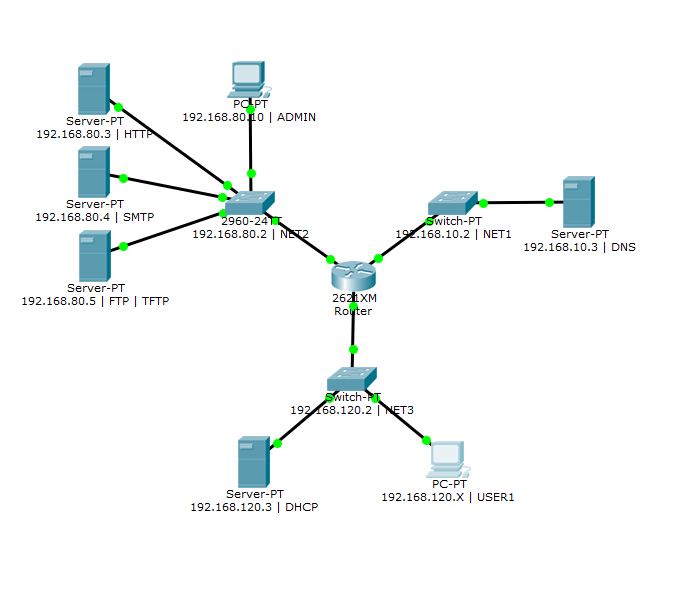
\includegraphics[scale = 0.58]{images/0.png}
	\caption{Результирующая схема ККС}
	\label{image:0}
\end{figure}

\section{Настройка сети}


\subsection{Настройка подсети NET1}

Конфигурация узлов подсети NET1 представлена на рис. \ref{image:1_1}.

\begin{figure}[h!]
	\centering
	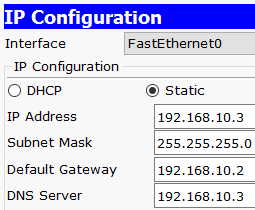
\includegraphics[scale = 0.64]{images/1_1.png}
	\caption{Настройка узла 192.168.10.3 (DNS сервер)}
	\label{image:1_1}
\end{figure}

\subsection{Настройка подсети NET2}

Конфигурация узлов подсети NET2 представлена на рис. \ref{image:2_1} -- \ref{image:2_4}.

\begin{figure}[h!]
	\centering
	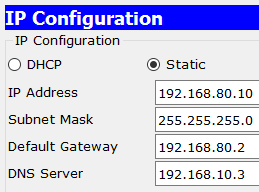
\includegraphics[scale = 0.64]{images/2_1.png}
	\caption{Настройка узла 192.168.80.10 (компьютер администратора)}
	\label{image:2_1}
\end{figure}

\begin{figure}[h!]
	\centering
	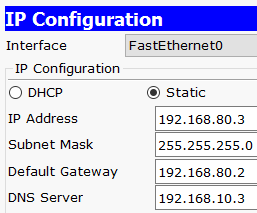
\includegraphics[scale = 0.64]{images/2_2.png}
	\caption{Настройка узла 192.168.80.3 (HTTP сервер)}
	\label{image:2_2}
\end{figure}

\begin{figure}[h!]
	\centering
	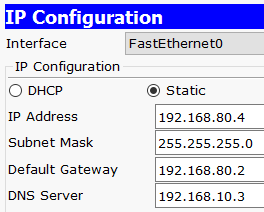
\includegraphics[scale = 0.65]{images/2_3.png}
	\caption{Настройка узла 192.168.80.4 (SMTP сервер)}
	\label{image:2_3}
\end{figure}

\begin{figure}[h!]
	\centering
	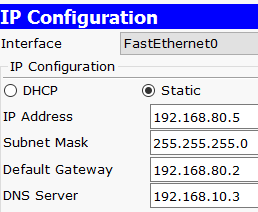
\includegraphics[scale = 0.65]{images/2_4.png}
	\caption{Настройка узла 192.168.80.5 (FTP/TFTP сервер)}
	\label{image:2_4}
\end{figure}

\subsection{Настройка подсети NET3}

Конфигурация узлов подсети NET3 представлена на рис. \ref{image:3_1} -- \ref{image:3_2}.

\begin{figure}[h!]
	\centering
	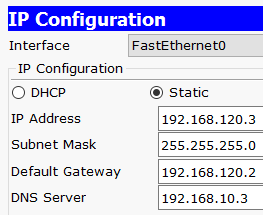
\includegraphics[scale = 0.65]{images/3_1.png}
	\caption{Настройка узла 192.168.120.3 (DHCP сервер)}
	\label{image:3_1}
\end{figure}

\begin{figure}[h!]
	\centering
	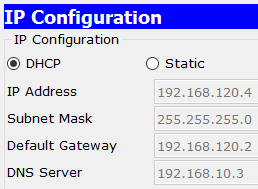
\includegraphics[scale = 0.65]{images/3_2.png}
	\caption{Настройка узла 192.168.120.X (компьютер пользователя)}
	\label{image:3_2}
\end{figure}

\subsection{Настройка роутера}

Конфигурация роутера представлена на рис. \ref{image:4_1} -- \ref{image:4_4}.

\begin{figure}[h!]
	\centering
	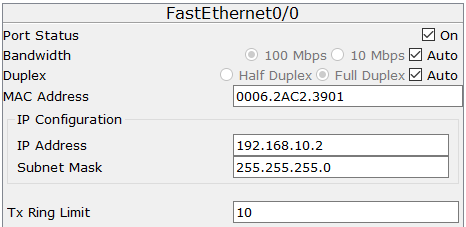
\includegraphics[scale = 0.65]{images/4_1.png}
	\caption{Настройка шлюза 192.168.10.2}
	\label{image:4_1}
\end{figure}

\begin{figure}[h!]
	\centering
	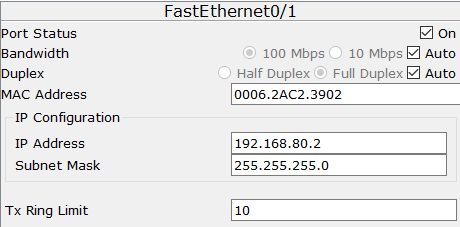
\includegraphics[scale = 0.65]{images/4_2.png}
	\caption{Настройка шлюза 192.168.80.2}
	\label{image:4_2}
\end{figure}

\begin{figure}[h!]
	\centering
	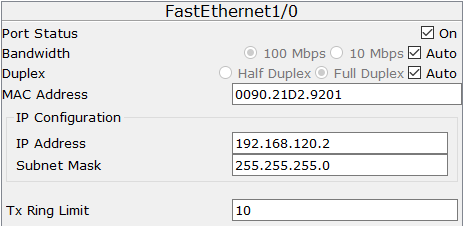
\includegraphics[scale = 0.65]{images/4_3.png}
	\caption{Настройка шлюза 192.168.120.2}
	\label{image:4_3}
\end{figure}

\begin{figure}[h!]
	\centering
	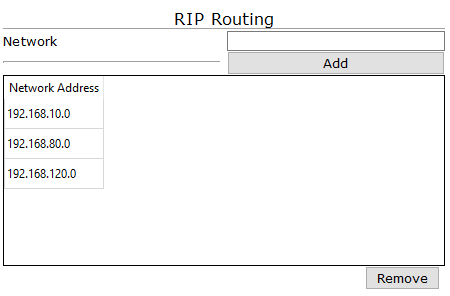
\includegraphics[scale = 0.65]{images/4_4.png}
	\caption{Маршрутизация}
	\label{image:4_4}
\end{figure}

\section{Настройка сетевых сервисов}

Конфигурация сетевых сервисов представлена на рис. \ref{image:5_1} -- \ref{image:5_6}.

\begin{figure}[h!]
	\centering
	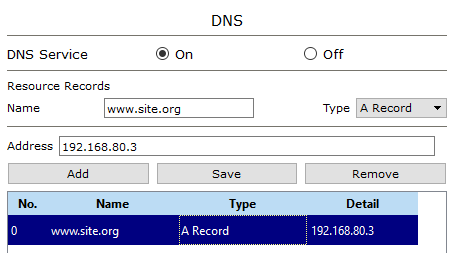
\includegraphics[scale = 0.74]{images/5_1.png}
	\caption{Настройка DNS сервера (192.168.10.3)}
	\label{image:5_1}
\end{figure}

\begin{figure}[h!]
	\centering
	
\includegraphics[scale = 0.82]{images/5_2.png}
	\caption{Настройка DHCP сервера (192.168.120.3)}
	\label{image:5_2}
\end{figure}

\begin{figure}[h!]
	\centering
	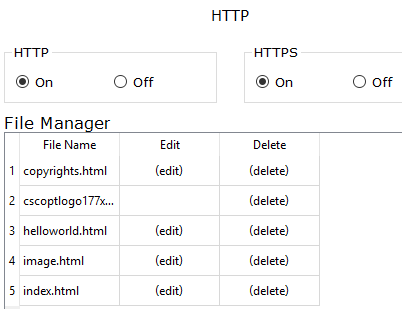
\includegraphics[scale = 0.82]{images/5_3.png}
	\caption{Настройка HTTP сервера (192.168.80.3)}
	\label{image:5_3}
\end{figure}

\begin{figure}[h!]
	\centering
	
\includegraphics[scale = 0.82]{images/5_4.png}
	\caption{Настройка SMTP сервера (192.168.80.4)}
	\label{image:5_4}
\end{figure}

\clearpage

\begin{figure}[h!]
	\centering
	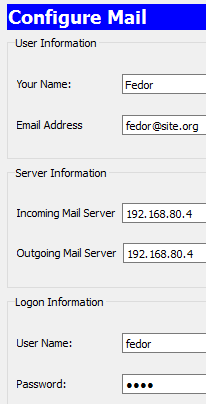
\includegraphics[scale = 0.76]{images/5_4_1.png}
	\caption{Настройка SMTP клиента (администратор Федор 192.168.80.10)}
	\label{image:5_4_1}
\end{figure}

\begin{figure}[h!]
	\centering
	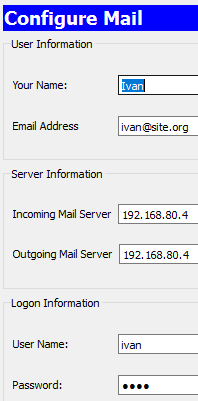
\includegraphics[scale = 0.76]{images/5_4_2.png}
	\caption{Настройка SMTP клиента (пользователь Иван 192.168.120.X)}
	\label{image:5_4_2}
\end{figure}

\begin{figure}[h!]
	\centering
	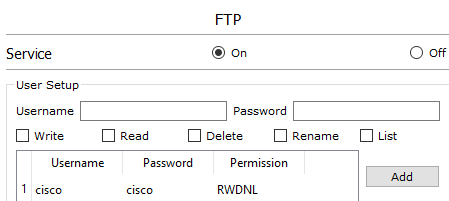
\includegraphics[scale = 0.83]{images/5_5.png}
	\caption{Настройка FTP сервера (192.168.80.5)}
	\label{image:5_5}
\end{figure}

\begin{figure}[h!]
	\centering
	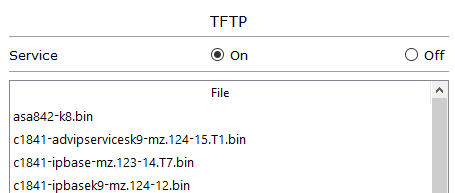
\includegraphics[scale = 0.89]{images/5_6.png}
	\caption{Настройка TFTP сервера (192.168.80.5)}
	\label{image:5_6}
\end{figure}

\section{Тестирование сети}

Тестирование доступности подсетей NET1 и NET2 из узла пользователя 192.168.120.X представлено на рис. \ref{image:6_1}.

\begin{figure}[h!]
	\centering
	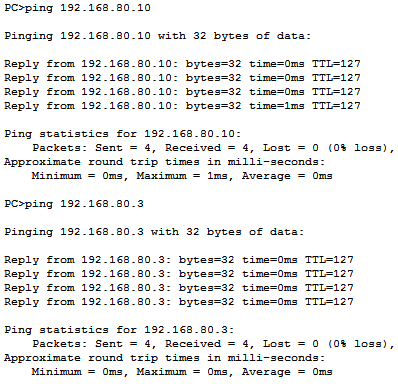
\includegraphics[scale = 0.89]{images/6_1.png}
	\caption{Тестирование доступности подсетей}
	\label{image:6_1}
\end{figure}

\clearpage

Тестирование работы DNS и HTTP серверов представлено на рис. \ref{image:6_2}.

\begin{figure}[h!]
	\centering
	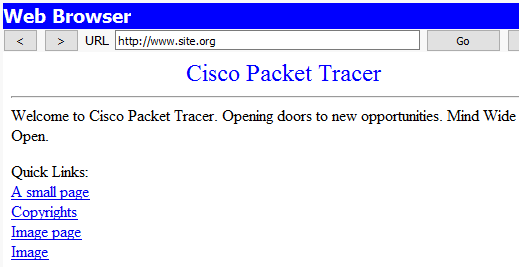
\includegraphics[scale = 0.75]{images/6_2.png}
	\caption{Тестирование работы DNS и HTTP серверов}
	\label{image:6_2}
\end{figure}

Отправление электронного письма от пользователя Ивана (192.168.120.X) к администратору Федору (192.168.80.10) представлено на рис. \ref{image:6_3_1}.

\begin{figure}[h!]
	\centering
	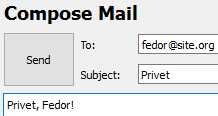
\includegraphics[scale = 0.95]{images/6_3_1.png}
	\caption{Отправление электронного письма}
	\label{image:6_3_1}
\end{figure}

Администратор Федор (192.168.80.10) успешно получил письмо (рис. \ref{image:6_3_2}).

\begin{figure}[h!]
	\centering
	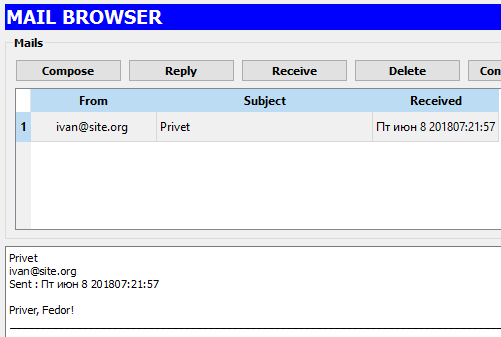
\includegraphics[scale = 0.95]{images/6_3_2.png}
	\caption{Получение электронного письма}
	\label{image:6_3_2}
\end{figure}

\clearpage

Тестирование работы FTP сервера представлено на рис. \ref{image:6_4}.

\begin{figure}[h!]
	\centering
	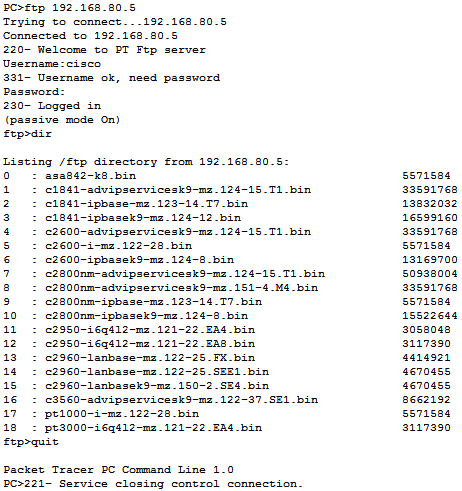
\includegraphics[scale = 0.85]{images/6_4.png}
	\caption{Тестирование работы FTP сервера}
	\label{image:6_4}
\end{figure}